\documentclass[aspectratio=169, ignorenonframetext]{beamer}
\usepackage{pgf}

\mode<article>{
  \usepackage{fullpage}

}

\mode<presentation>
{
%   \usetheme{Madrid}
%   \useinnertheme{circles}
  \setbeamertemplate{navigation symbols}{}
%   \usetheme[hideothersubsections, width=2.4cm]{Hannover}
%   \usetheme{Antibes}
%   \usetheme{Montpellier}
  \usetheme{Singapore}
%   \usecolortheme{seahorse}
  \setbeamertemplate{footline}
  {%
%     \begin{beamercolorbox}{section in head/foot}
%       \usebeamercolor{bg}
       \hskip 1em \footnotesize \insertframenumber{} / \inserttotalframenumber%\hskip 41em 
\includegraphics[height = .5cm]{../../../../bilder/cc_by-nc_eu.png}
% % cc_by-nc_eu.png: 403x141 px, 72dpi, 14.22x4.97 cm, bb=0 0 403 141
%
% % bwslogo_3.png: 476x392 px, 300dpi, 4.03x3.32 cm, bb=0 0 114 94
%
%       %\hskip 5em
%       %       \input{../bilder/cc_by.png}
%       %\includegraphics[height=.5cm]{../../../../bilder/bwslogo_3.png}
%     \end{beamercolorbox}%
  }
  \usepackage{beamerfoils}
}
\usepackage[german]{babel}
\usepackage[utf8]{inputenc}
\usepackage{times}
\usepackage[T1]{fontenc}
\usepackage{pgf}
\usepackage{pgfpages}
\usepackage{eurosym}
\usepackage{graphicx}
\usepackage{amsmath}
\usepackage[siunitx,european]{circuitikz}
% \usepackage{ulem}
\usepackage{listings}
\usepackage{svg}
%
\lstset{numbers=left, numberstyle=\tiny, stepnumber=2, numbersep=5pt, language = C++, alsolanguage=XML}
% \MyLogo{\includegraphics[height=1cm]{../../../../bilder/bwslogo_3.png}}
% % \includegraphics{../../bilder/bwslogo_3.png}
% % bwslogo_3.png: 476x392 px, 300dpi, 4.03x3.32 cm, bb=
%
\only<article>{
  \usepackage[colorlinks=true,linkcolor=blue,filecolor=magenta,urlcolor=cyan]{hyperref}
}

\only<presentation>{
  \usepackage{hyperref}
}


\title{Aufgabe - Schaltung 3}
% \date{V 0.2.1 - im Aufbau\\ Stand: \today}%\\

\institute[BWS Hofheim]{Brühlwiesenschule, Hofheim}
\author{Thomas Maul}

\AtBeginSection[] % Do nothing for \section*
{
  \begin{frame}<beamer>
    \frametitle{Inhalt}
    \tableofcontents[currentsection]
  \end{frame}
}

\begin{document}

\begin{frame}{Aufgabe}
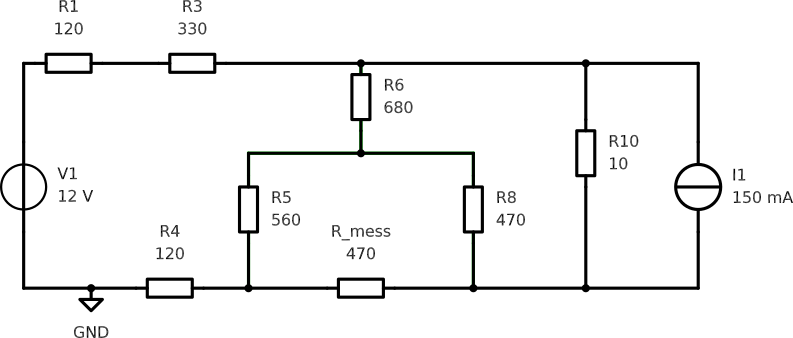
\includegraphics{bruecke2/bruecke2a/schaltung3_1.png}

Berechnen Sie den Strom und die Spannung am Widerstand R-Mess.

Verwenden Sie das Maschenstromverfahren oder das Überlagerungs-Verfahren. Wandeln Sie ggf. Widerstände in Dreiecks-Konfiguration in einen Stern um oder Widerstände in Stern-Konfiguration in ein Dreieck.
\end{frame}

\begin{frame}{Vollständiger Baum}
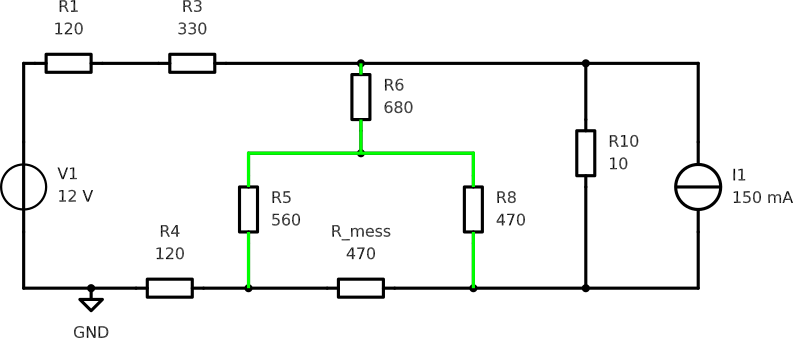
\includegraphics{bruecke2/bruecke2a/schaltung3_2.png}
\end{frame}

\begin{frame}{Knoten markiert}
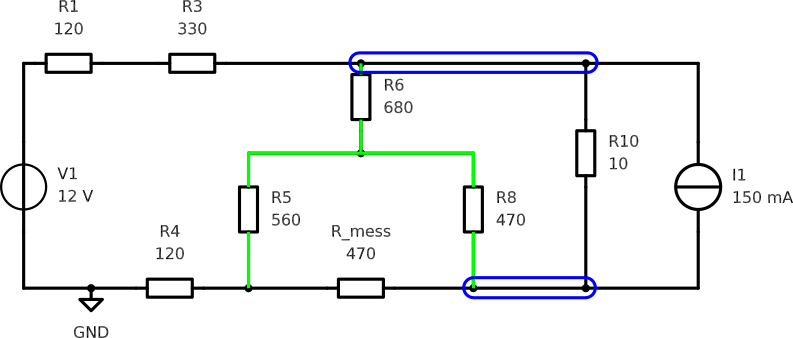
\includegraphics{bruecke2/bruecke2a/schaltung3_3.png}
\end{frame}

\begin{frame}{Stromquelle umwandeln}
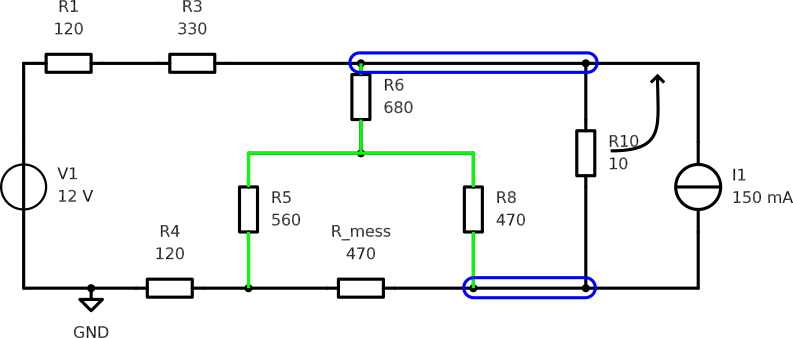
\includegraphics{bruecke2/bruecke2a/schaltung3_4.png}
\end{frame}

\begin{frame}{Stromquelle umgewandelt}
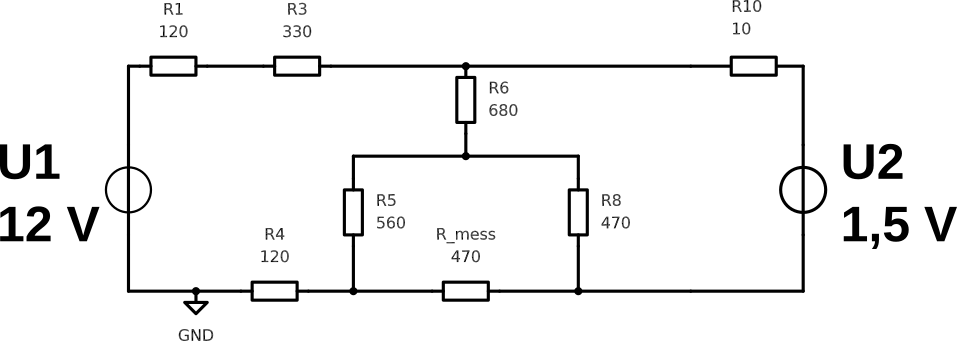
\includegraphics{bruecke2/bruecke2a/schaltung3_1a.png}
\end{frame}

\begin{frame}{Maschen}
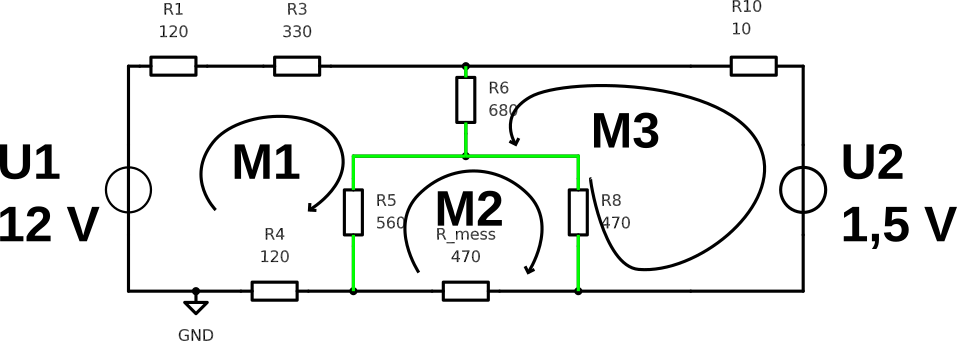
\includegraphics{bruecke2/bruecke2a/schaltung3_2a.png}
\end{frame}



\label{LastPage}
\end{document}
